\documentclass{beamer}

\usepackage{amssymb,amsmath}
\usepackage{graphicx}
\usepackage{url}
\usepackage{color}
\usepackage{relsize}		% For \smaller
\usepackage{url}			% For \url
\usepackage{epstopdf}	% Included EPS files automatically converted to PDF to include with pdflatex

%For MindMaps
% \usepackage{tikz}%
% \usetikzlibrary{mindmap,trees,arrows}%

%%% Color Definitions %%%%%%%%%%%%%%%%%%%%%%%%%%%%%%%%%%%%%%%%%%%%%%%%%%%%%%%%%
%\definecolor{bordercol}{RGB}{40,40,40}
%\definecolor{headercol1}{RGB}{186,215,230}
%\definecolor{headercol2}{RGB}{80,80,80}
%\definecolor{headerfontcol}{RGB}{0,0,0}
%\definecolor{boxcolor}{RGB}{186,215,230}

%%% Save space in lists. Use this after the opening of the list %%%%%%%%%%%%%%%%
%\newcommand{\compresslist}{
%	\setlength{\itemsep}{1pt}
%	\setlength{\parskip}{0pt}
%	\setlength{\parsep}{0pt}
%}

%\setbeameroption{show notes on top}

% You should run 'pdflatex' TWICE, because of TOC issues.

% Rename this file.  A common temptation for first-time slide makers
% is to name it something like ``my_talk.tex'' or
% ``john_doe_talk.tex'' or even ``discrete_math_seminar_talk.tex''.
% You really won't like any of these titles the second time you give a
% talk.  Try naming your tex file something more descriptive, like
% ``riemann_hypothesis_short_proof_talk.tex''.  Even better (in case
% you recycle 99% of a talk, but still want to change a little, and
% retain copies of each), how about
% ``riemann_hypothesis_short_proof_MIT-Colloquium.2000-01-01.tex''?

\mode<presentation>
{
  % A tip: pick a theme you like first, and THEN modify the color theme, and then add math content.
  % Warsaw is the theme selected by default in Beamer's installation sample files.

  %%%%%%%%%%%%%%%%%%%%%%%%%%%% THEME
  %\usetheme{AnnArbor}
  %\usetheme{Antibes}
  %\usetheme{Bergen}
  %\usetheme{Berkeley}		% bem bacana - menu esquerdo
  %\usetheme{Berlin}
  %\usetheme{Boadilla}
  %\usetheme{boxes}
  %\usetheme{CambridgeUS}		% bem bacana - menu superior
  %\usetheme{Copenhagen}
  %\usetheme{Darmstadt}
  %\usetheme{default}
  %\usetheme{Dresden}
  \usetheme{Frankfurt}
  %\usetheme{Goettingen}
  %\usetheme{Hannover}		% bem bacana - menu esquerdo
  %\usetheme{Ilmenau}
  %\usetheme{JuanLesPins}
  %\usetheme{Luebeck}
  %\usetheme{Madrid}		%bacana
  %\usetheme{Malmoe}
  %\usetheme{Marburg}		% bem bacana - menu direito
  %\usetheme{Montpellier}
  %\usetheme{PaloAlto}		% bem bacana - menu esquerdo
  %\usetheme{Pittsburgh}
  %\usetheme{Rochester}		%bacana
  %\usetheme{Singapore}
  %\usetheme{Szeged}
  %\usetheme{Warsaw}

  %%%%%%%%%%%%%%%%%%%%%%%%%%%% COLOR THEME
  %\usecolortheme{albatross}		% azul escuro, massa
  %\usecolortheme{beetle}		% cinza, menu azul
  %\usecolortheme{crane}		% branco e amarelo, massa
  \usecolortheme{default}		% branco, azul clarinho
  %\usecolortheme{dolphin}		% azul e branco, legal
  %\usecolortheme{dove}			% cinza e branco, feio
  %\usecolortheme{fly}			% todo cinza, horrível
  %\usecolortheme{lily}			% parece o default
  %\usecolortheme{orchid}		% azul e branco, ok
  %\usecolortheme{rose}			% branco e violeta-claro, bonito
  %\usecolortheme{seagull}		% cinza, feio
  %\usecolortheme{seahorse}		% nhé, meio feio
  %\usecolortheme{sidebartab}		% Azul, branco, destaque na tab, interessante
  %\usecolortheme{structure}		% bichado
  %\usecolortheme{whale}		% Azul e branco, bem bonito

  %%%%%%%%%%%%%%%%%%%%%%%%%%%% OUTER THEME
  \useoutertheme{default}
  %\useoutertheme{infolines}
  %\useoutertheme{miniframes}
  %\useoutertheme{shadow}
  %\useoutertheme{sidebar}
  %\useoutertheme{smoothbars}
  %\useoutertheme{smoothtree}
  %\useoutertheme{split}
  %\useoutertheme{tree}

  %%%%%%%%%%%%%%%%%%%%%%%%%%%% INNER THEME
  \useinnertheme{circles}
  %\useinnertheme{default}
  %\useinnertheme{inmargin}
  %\useinnertheme{rectangles}
  %\useinnertheme{rounded}

  %%%%%%%%%%%%%%%%%%%%%%%%%%%%%%%%%%%

  \setbeamercovered{invisible} % or whatever (possibly just delete it)
  % To change behavior of \uncover from graying out to totally
  % invisible, can change \setbeamercovered to invisible instead of
  % transparent. apparently there are also 'dynamic' modes that make
  % the amount of graying depend on how long it'll take until the
  % thing is uncovered.

}


% Get rid of nav bar
\beamertemplatenavigationsymbolsempty

% Use short top
%\usepackage[headheight=12pt,footheight=12pt]{beamerthemeboxes}
%\addheadboxtemplate{\color{black}}{
%\hskip0.5cm
%\color{white}
%\insertshortauthor \ \ \ \ 
%\insertframenumber \ \ \ \ \ \ \ 
%\insertsection \ \ \ \ \ \ \ \ \ \ \ \ \ \ \ \ \  \insertsubsection
%\hskip0.5cm}
%\addheadboxtemplate{\color{black}}{
%\color{white}
%\ \ \ \ 
%\insertsection
%}
%\addheadboxtemplate{\color{black}}{
%\color{white}
%\ \ \ \ 
%\insertsubsection
%}

% Insert frame number at bottom of the page.
% \usefoottemplate{\hfil\tiny{\color{black!90}\insertframenumber}} 

\usepackage[english]{babel}
\usepackage[latin1]{inputenc}
\usepackage{subfigure}

\usepackage{times}
\usepackage[T1]{fontenc}


\title[GB21802]{GB21802 - Programming Challenges}
\subtitle[]{Week 1 - Data Structures}
\author[Claus Aranha]{Claus Aranha\\{\footnotesize caranha@cs.tsukuba.ac.jp}}
\institute{College of Information Science}
\date{2019-04-19,22\\{\tiny Last updated \today}}

\begin{document}

\begin{frame}
\maketitle
\end{frame}

\section{Last Week}
\subsection{Notes Previous Class}

\begin{frame}
  \frametitle{Results for the Previous Week}

  \begin{center}
    Here are the results for last week:

    \bigskip
    
    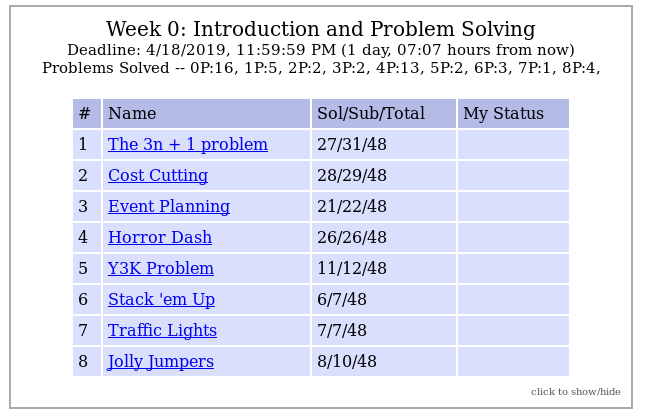
\includegraphics[width=0.8\textwidth]{img/resultW0}
    
    \bigskip

    Hope you enjoyed the warm up!
  \end{center}

\end{frame}

\begin{frame}[fragile]
  \frametitle{Comments from e-mails and questions -- 1}

  \begin{block}{Submission with Java}
    Two students had \structure{``runtime error''} with Java last week
    -- don't forget that your start class MUST be called {\bf Main}.
  \end{block}

  \vfill

\begin{verbatim}
class Main {
  public static void main(String[] args) {

    // do something...

  }
}
\end{verbatim}
\end{frame}

\begin{frame}
  \frametitle{Comments from e-mails and questions -- 2}
  \begin{block}{Input/Output}
    Two other students had problems because their program printed ``Please enter a number''.

    \bigskip

    You are very kind, but please {\bf follow the specifications} strictly!
  \end{block}
  
  \vfill

  \begin{block}{Format for MANABA submission}
    One student asked if the code for MANABA had to be the same as the code for UVA.

    \bigskip

    Yes. The code you submit on MANABA must be {\bf exactly the same}
    as the code you submitted for UVA.
  \end{block}
\end{frame}

\begin{frame}
  \frametitle{Short comments about the problems:}
  \begin{itemize}
  \item Cost Cutting, Event Planning, Horror Dash -- Easiest problems (find mean, find min, find min);
    \bigskip

  \item 3n+1 -- Still easy, but a few traps -- example of {\bf Memoization};
    \bigskip

  \item Y3K Problem -- Still easy, but skip year can be a bit troublesome.
    
  \end{itemize}
\end{frame}

%\begin{frame}
%  \frametitle{Comments about the problems}
%\end{frame}


\section{Introduction}
\begin{frame}
  \frametitle{}

  \begin{center}
    {\large Data Structures}\\
    CP Book Chapter 2
  \end{center}
\end{frame}

\subsection{Outline}
\begin{frame}
  \frametitle{Data Structures and Programming Challenges}

  \begin{itemize}
    \item Using the correct data structure makes the \alert{program faster}.
    \bigskip

    \item Using the correct data structure makes the \alert{problem easier}.
    \bigskip

    \item Every program needs \alert{some} data structure. Learn it!
  \end{itemize}

  \vfill

  \begin{block}{}
    In this lecture, we review some common data structures, and we
    also look a bit at \structure{common library functions}
  \end{block}
\end{frame}

\begin{frame}[fragile]
  \frametitle{Example 0: 8 Queen Problem (UVA 750)}
  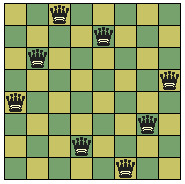
\includegraphics[width=0.25\textwidth]{../img/8queen}\\

  For a board of size $n \times n$, find \alert{how many} safe
  configurations of $n$ queens exist.

  \bigskip

  Because we need to find \alert{how many} configurations exist,
  we need to test ``all'' configurations.

  \bigskip

\begin{verbatim}
for i = 0 to #configurations do
  sum = testIfConfigurationIsSafe(i)
\end{verbatim}

  {\tiny\hfill Image by Lee Daniel Crocker. CC-BY-SA 3.0}
\end{frame}

\begin{frame}[fragile]
  \frametitle{Example 0: 8 Queen Problem (UVA 750)}

How can we represent a configuration?

\bigskip

(1) Position $x,y$ of every queen (size: $n^{n^2}$)
\begin{verbatim}
conf[0] = {{a,1}, {a,1}, {a,1}, ... {a,1}, {a,1}}
conf[1] = {{a,1}, {a,1}, {a,1}, ... {a,1}, {a,2}}
conf[2] = {{a,1}, {a,1}, {a,1}, ... {a,1}, {a,3}}
\end{verbatim}
\bigskip

(2) Row $r$ of every queen (size: $n^n$)
\begin{verbatim}
conf[0] = {0,0,0,0,0,0,0,0}
conf[1] = {0,0,0,0,0,0,0,1}
conf[2] = {0,0,0,0,0,0,0,2}
\end{verbatim}

(3) Permutation of row positions (size: $n!$)
\begin{verbatim}
conf[0] = {0,1,2,3,4,5,6,7}
conf[1] = {0,1,2,3,4,5,7,6}
conf[2] = {0,1,2,3,4,6,5,7}
\end{verbatim}
\end{frame}

\begin{frame}
  \frametitle{Example 1: The Towers of Hanoi}

  \begin{center}
    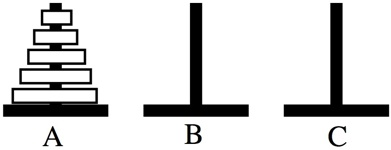
\includegraphics[width=0.5\textwidth]{img/hanoi}
  \end{center}
  \medskip

  {\small
    \begin{itemize}
    \item You have $N$ disks and $K$ poles. Each disk has unique size $s_i$.
    \item A disk $i$ can be moved from one pole to another.
    \item A move of disk $i$ to pole $k$ is only valid if $k$ has no disks smaller than $i$
    \item Find the list of moves to move all disks from pole 1 to pole $K$.
    \end{itemize}
  }

  \vfill

  How do you represent the data in this problem?
\end{frame}

\begin{frame}
  \frametitle{Example 1: The Towers of Hanoi}
  A string with ``n'' disks, from smaller to larger.
  \begin{center}
    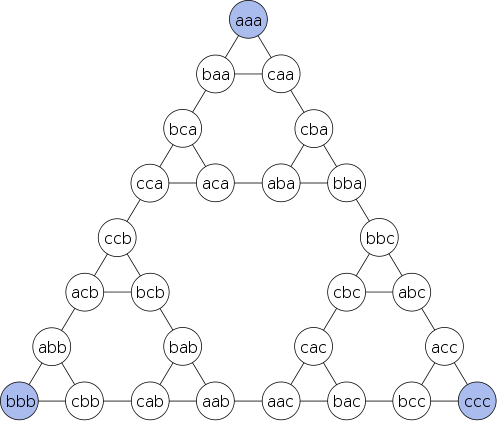
\includegraphics[width=0.65\textwidth]{img/hanoi_graph}
  \end{center}
  {\tiny \hfill Image created by nonenmac}
\end{frame}

\subsection{Example 3 -- Army Buddies}

\begin{frame}[fragile]
  \frametitle{Example 2: Army Buddies (UVA 12356)}
  \framesubtitle{Problem Description}

  \begin{block}{}
    \begin{itemize}
    \item There is a line of $S$ soldiers: $0,1,2,3,4,...,S$
    \item There are $Q$ queries that remove soldiers from $i$ to $j$:
\begin{verbatim}
Q1: 2,4           (removes soldiers 2, 3, 4)
Q2: 6,7           (removes soldiers 6, 7)
Q3: 1,1           (removes soldier 1)
\end{verbatim}
    \item For each query, list the soldier to the \alert{left} and to the \alert{right}
\begin{verbatim}
A1: 1,5       1 x x x 5 6 7
A2: 5,*       1 - - - 5 x x
A3: *,5       x - - - 5 - -
\end{verbatim}
    \end{itemize}
  \end{block}

  \bigskip

  How do we solve this problem?
\end{frame}

\begin{frame}
  \frametitle{Example 2: Army Buddies (UVA 12356)}
  \framesubtitle{Idea 1: Linked Lists}

  \begin{center}
    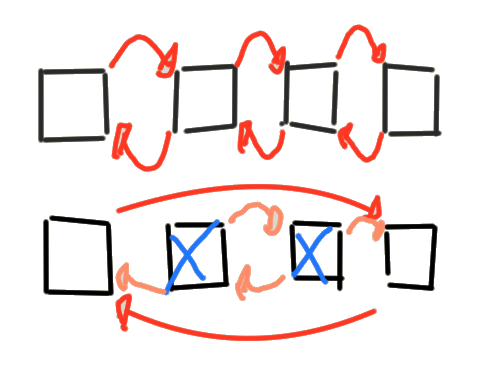
\includegraphics[width=0.5\textwidth]{img/army-list}
  \end{center}

  \begin{itemize}
  \item Represent the line as a linked list.
  \item Find the 1\textsuperscript{st} soldier \hfill \structure{(This is $O(n)$)}
  \item Find the 2\textsuperscript{nd} soldier \hfill \structure{(This is $O(n)$)}
  \item Update the list and print the neighbors. \hfill \structure{(This is $O(1)$)}
  \end{itemize}
  \bigskip

\end{frame}

\begin{frame}
  \frametitle{Example 2: Army Buddies (UVA 12356)}
  \framesubtitle{A solution using linked lists}

  \begin{center}
    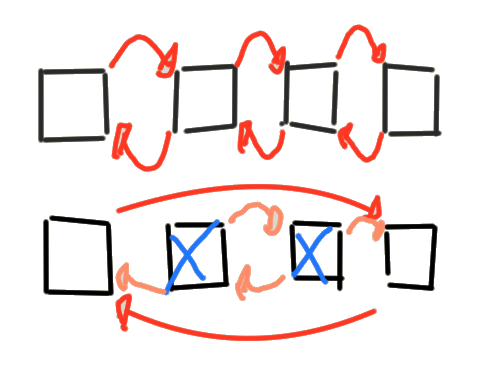
\includegraphics[width=0.4\textwidth]{img/army-list}
  \end{center}

  \alert{Problem!} The input is too big, and O(n) takes too much time.

  \begin{itemize}
  \item $1 \leq S \leq B \leq 10^5$;\hfill \structure{($O(n^2)) = 10^{10}$}
  \item Also \alert{multiple cases};\hfill \structure{($O(n^2k)) = 10^{10}k$}
  \end{itemize}

  \bigskip

  Think of a different solution! (Do not look at the next slide :-))
\end{frame}


\begin{frame}[t]
  \frametitle{Example 2: Army Buddies (UVA 12356)}
  \framesubtitle{A solution using arrays}

  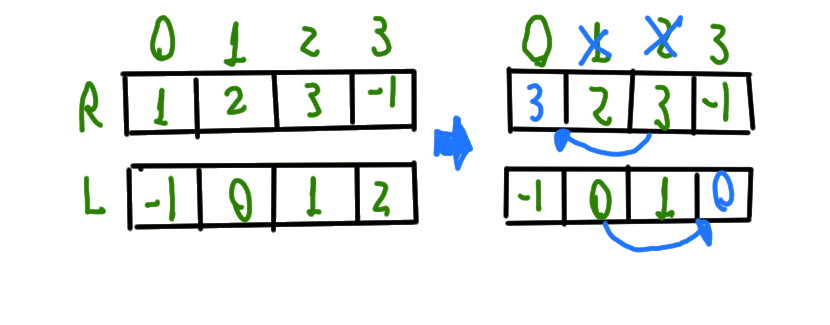
\includegraphics[width=0.8\textwidth]{img/army-array}

  \begin{itemize}
  \item \alert{Problem}: Do not update ALL soldiers, just the edge.
  \item \structure{Idea}: Neighbor Array
    \begin{itemize}
    \item Let {\bf R} be: {\bf Int} Array of Right neighbors
    \item Let {\bf L} be: {\bf Int} Array of Left neighbors
    \end{itemize}
  \item \structure{Question}: how do we update R and L after query $(r,l)$?\\
  \end{itemize}
\end{frame}

\subsection{Thinking about Data Structures}
\begin{frame}
  %% TODO: Improve this frame
  \frametitle{Data Structures and Programming Contests}
  \begin{itemize}
    \item Choosing the right data structure makes the program \structure{easy and fast}

    \vfill

    \item Always avoid pointers \alert{in programming contests}
    \begin{itemize}
      \item Too many bugs
      \item Not enough gains
      \item Better to use arrays!
    \end{itemize}

    \bigskip

    \item \structure{Remember the STL} for common data structure!
  \end{itemize}
\end{frame}


\section{Linear Data Structures}
\subsection{Basics}

\begin{frame}
  \frametitle{The simple array!}
  Arrays are the simplest data structure, but also the most often used.

  \bigskip

  \structure{Merits}
  \begin{itemize}
  \item Easy to implement! No worries about pointers;
  \item Can simulate pointers using index operations;
  \item Many library Functions;
  \end{itemize}

  \bigskip

  \alert{Concerns}
  \begin{itemize}
  \item Reordering many items can be expensive;
  \end{itemize}
\end{frame}


\begin{frame}[fragile]
  \frametitle{Implementing arrays/vectors (C++)}
  {\small
\begin{verbatim}
#include <vector>

int arr[5] = {7,7,7};     // arr = {7,7,7,0,0}
vector<int> v(5, 5);      // v = {5,5,5,5,5}

int x = arr[2] + v[2];    // x = 12

arr[5] = 5;               // Runtime error
cout << v[7];             // 0 !! Be careful.

v.push_back(6);           // v = {5,5,5,5,5,6}
\end{verbatim}
  }

  \begin{alertblock}{}
    Trying to access indexes outside of an array is a common source of
    Runtime Errors (RTE)
  \end{alertblock}

\end{frame}

\begin{frame}[fragile]
  \frametitle{How do you reset an array?}
  \framesubtitle{Implementation matters}
{\small
\begin{verbatim}
#include <vector>
#include <string.h>
vector<int> v(10000,7)

memset(v, 0, 10000*__SIZEOF_INT__);       // Method 1
fill(v.begin(), v.end(), 0);              // Method 2
for (int i = 0; i < 10000; i++) v[i] = 0; // Method 3
v.assign(v.size(), 0);                    // Method 4


Method      |  executable size  |  Time Taken (in sec) |
            |  -O0    |  -O3    |  -O0      |  -O3     |
------------|---------|---------|-----------|----------|
1. memset   | 17 kB   | 8.6 kB  | 0.125     | 0.124    |
2. fill     | 19 kB   | 8.6 kB  | 13.4      | 0.124    |
3. manual   | 19 kB   | 8.6 kB  | 14.5      | 0.124    |
4. assign   | 24 kB   | 9.0 kB  | 1.9       | 0.591    |
\end{verbatim}
}
\end{frame}

\subsection{Sorting and Searching}

\begin{frame}
  \frametitle{Operations in Arrays}

  \begin{block}{Example -- Vito's Family (UVA 10041)}
    {\bf Input:} A list of integers (street addresses):\\

    \smallskip

    10, 20, 10, 10, 40, 80, 30, 90, 20, 55, 20

    \bigskip

    {\bf Output:} The address (integer) with \structure{minimal} distance to all others.
    \begin{itemize}
      \item {\bf 10}: $0+10+0+0+30+70+20+80+10+45+10 = 275$
      \item {\bf 40}: $30+20+30+30+0+40+10+50+20+15+20 = 265$
      \item {\bf 20}: $10+0+10+10+20+60+10+70+0+35+0 = 225$
    \end{itemize}

    \bigskip

    Result: 20!

  \end{block}

  \bigskip

  How do we solve this problem?

\end{frame}

\begin{frame}[fragile]
  \frametitle{Operations in Arrays}

  \begin{itemize}
  \item Solution: Find the \structure{Median} address.
  \item 1- \structure{sort the address array}, 2- select the middle value.
  \end{itemize}

\begin{verbatim}
  #include<iostream>
  #include<algorithm>
  using namespace std;

  int main() {
      int n; int add[100];
      cin >> n;
      for (int i=0; i<n; i++) { cin >> add[i]; }

      sort(add, add+n);

      cout << add[n/2] << endl;
  }
\end{verbatim}
\end{frame}

\begin{frame}
  \frametitle{Using Sorting}
  Sorting can be used for \alert{many, many} things:

  \bigskip

    \begin{itemize}
    \item Finding the Highest $n$ values, Finding duplicate values;
      \bigskip

    \item Binary Search ($O(\log n)$)
      \bigskip

    \item Pre-processing data for other algorithms.
    \end{itemize}

  \bigskip
  Let's do Sorting!
\end{frame}

\begin{frame}[fragile]
  \frametitle{algorithm, sorting and binary search}
{\small
\begin{block}{}
\begin{verbatim}
#include <iostream>
#include <algorithm>
#include <vector>
using namespace std;

int main () {
  int n, t, search; vector<int> v;
  cin >> n >> search;
  for (int i=0; i<n; i++) { cin >> t; v.push_back(t); }

  sort (v.begin(), v.end());
  vector<int>::iterator low,up;
  low = lower_bound (v.begin(), v.end(), search);
  up  = upper_bound (v.begin(), v.end(), search);
  cout << (low-v.begin()) << " and " << (up-v.begin());
}
\end{verbatim}
\end{block}}
\end{frame}


\begin{frame}[fragile]
  \frametitle{Sorting with specific sorting function}
{\small
  Imagine you need to sort by number of points (bigger is best),
  penalty (smaller is best), and name (alphabetical order)

  \begin{block}{}
\begin{verbatim}
#include <algorithm>
#include <vector>
#include <string>
struct team{ string name; int point; int penal;
             team(string _n, int _po, int _pe) :
               name(_n), point(_p), penal(_g){} };

bool cmp(team a, team b) {
  if (a.point != b.point) return a.point > b.point;
  if (a.penal != b.penal) return a.penal < b.penal;
  return strcmp(a.name,b.name); }

vector<team> v;
sort(v.begin(), v.end(), cmp); // sort using cmp
reverse(v.begin(), v.end()); // and reverse
\end{verbatim}
\end{block}}
\end{frame}

\subsection{Bitmask}

\begin{frame}
  \frametitle{A Permutation Problem}
  \begin{itemize}
    \item \structure{Input}: A set of item costs: $c_1, c_2, c_3, \ldots, c_n$, and your money $m$.
    \bigskip

    \item \structure{Output}: The list of indexes of items you can buy.
    \bigskip

    \item \structure{how to do it?}: Test all possible \alert{item permutations}
    \bigskip

    \item But how?
  \end{itemize}
\end{frame}

\begin{frame}[fragile]
  \frametitle{Looping Permutations}

{\small
  \begin{block}{}
\begin{verbatim}
#include <iostream>
#include <vector>
using namespace std;

int main () {
  int n, t, m; vector<int> p;
  cin >> n >> m;
  for (int i=0; i<n; i++)
    { cin >> t; p.push_back(t); }

  for (int i = 0; i < (1 << n); i++) {
      t = 0;
      for (int j = 0; j < n; j++)
          t += (i & (1 << j) ? p[j] : 0);
      if (t == m)
          cout << "found!" << endl;
}}
\end{verbatim}
\end{block}}
\end{frame}

\begin{frame}[fragile]
  \frametitle{Bitmasks}

\begin{block}{}
\begin{verbatim}
1 --> for (int i = 0; i < (1 << n); i++) {
2 --> t += (i & (1 << j) ? p[j] : 0);
\end{verbatim}
\end{block}

\begin{itemize}
  \item Bitmasks are \structure{sets of booleans} using \alert{integers}.
  \bigskip

  \item They are very useful for representing \alert{sets}
  \begin{itemize}
    \item Set Looping;
    \item Set Union (OR);
    \item Set Intersection (AND);
  \end{itemize}
  \bigskip

  \item They are \structure{Very fast too}
  \end{itemize}
\end{frame}

\begin{frame}[fragile]
  \frametitle{Binary Operatons on Bitmasks (2)}
{\smaller

  \begin{itemize}
  \item Multiply/Divide an integer by two :: shift bits left, right
\begin{verbatim}
S                = 34 =  100010
S = S << 1 = S*2 = 68 = 1000100
S = S >> 2 = S/4 = 17 =   10001
S = S >> 1 = S/2 =  8 =    1000
\end{verbatim}
\bigskip

\item Check if the i-th bit is turned on:
\begin{verbatim}
S          = 34       =  100010
j = 3, 1 << j         =  001000
i = 1, 1 << 1         =  000010
                         ------
Tj= S & ( 1 << j)     =  000000  = 0 # 3 is not set
Ti= S & ( 1 << i)     =  000010 != 0 # 1 is set
\end{verbatim}

  \end{itemize}

}
\end{frame}

\begin{frame}[fragile]
  \frametitle{Binary Operations on Bitmasks (2)}
  {\smaller
  \begin{itemize}
  \item To set/turn on the jth item, use bitwise OR operation S |= (1 << j)
\begin{verbatim}
S          = 34       =  100010
j = 3, 1 << j         =  001000
                         ------ OR (S |= 1 << j)
S          = 42       =  101010
\end{verbatim}
\item To set/turn off the jth item, use bitwise AND operation S \&= ~(1 << j)
\begin{verbatim}
S          = 50       =  110010
j = (1<<5)|(1<<3)     =  101000 # unset items 5,3
~j                    =  010111
                         ------
S &= ~(j)             =  010010 # 18
\end{verbatim}
\bigskip

\item There is the \structure{bitset} class, but it cannot be used as an
\structure{array index}.

  \end{itemize}

  }
\end{frame}



\section{Library Structures}

\subsection{Visalgo}
\begin{frame}
  \frametitle{Long Live the STL!}

  \begin{itemize}
    \item The standard library implements many data structures that are
      useful for programming contests.
      \bigskip

    \item Let's review a few of them here.
      \bigskip

    \item The website \url{https://visualgo.net/} has good reviews of many
     data structures;
  \end{itemize}

\end{frame}

%%%%%%%%%%%%%%%%%%%%%%%%%%%%%%%%%%%%%%%%%%%%%%%%%%%%%%%%%
\subsection{Deque, Queue, Stack}

%% TODO: Add Motivating Problem For Queue
\begin{frame}
  \frametitle{Deque, Queue, Stack}

  Sometimes you want special access to the \structure{start} or \structure{end}
  of a vector.

  \bigskip

  \begin{itemize}
    \item \structure{stack}: \emph{pop} and \emph{push} from the front;
    \bigskip

    \item \structure{queue}: \emph{pop} from the back, \emph{push} from the front;
    \bigskip

    \item \structure{deque}: \emph{pop\_front, push\_front, pop\_back, push\_back};
  \end{itemize}
  \bigskip

  \begin{block}{Behind C++}
    Actually, \emph{Queue} and \emph{Stack} are high level constructs,
    \structure{List} or \structure{Deque} are used to implement them.
  \end{block}
\end{frame}

\begin{frame}[fragile]
  \frametitle{Queue and Stacks}

  \begin{block}{}
    Queues and Stacks are useful to simplify common cases of vectors
  \end{block}

  Stack Example: Testing if a set of parenthesis is balanced.
{\small
\begin{verbatim}
#include <stack>
stack<char> s;
char c;

while(cin >> c) {
  if (c == '(') s.push(c);
  else {
    if (s.size() == 0) { s.push('*'); break; }
    s.pop();
  }
}
cout << (s.size() == 0 ? "balanced" : "unbalanced");

\end{verbatim}}
\end{frame}


\subsection{Balanced Search Tree (BST) -- Maps and Sets}

\begin{frame}
  \frametitle{Problem Example: CD -- 11849}

  \begin{block}{}
    {\bf Input:}
    \begin{itemize}
    \item Jack CD collection: Up to $10^6$ CDs, with ID up to $10^9$
    \item Jill CD collection: Up to $10^6$ CDs, with ID up to $10^9$
    \end{itemize}

    {\bf Output:}
    \begin{itemize}
    \item How Many CDs are in both Collections?
    \end{itemize}

  \end{block}
\end{frame}

\begin{frame}
  \frametitle{Problem Example: CD -- 11849}

  Naive Solution:

  \begin{enumerate}
  \item Store all IDs in collection 1 in a Vector (n)
  \item Sort the Vector (nlogn)
  \item For each ID in collection 2, test if it exists in Vector with \structure{Binary Search} (nlogn)
  \end{enumerate}

  Total Cost: $n + n\text{log}n + n\text{log}n$

  \bigskip

  Let's use a \structure{MAP} for $O(\log N)$ search using a \structure{balanced search tree}
\end{frame}

\begin{frame}[fragile]
  \frametitle{Solving CD with a MAP (Approximate Solution)}

{\smaller
  \begin{block}{}
\begin{verbatim}
#include <iostream>
#include <set>
using namespace std;

int main() {
    int N, M, num;
    cin >> N >> M;

    set<int> first, second;
    while (N--) { cin >> num; first.insert(num); }
    while (M--) { cin >> num; second.insert(num); }
    int count = 0;
    for (set<int>::iterator iter = first.begin();
         iter != first.end(); ++iter)
      if (second.find(*iter) != second.end())
        ++count;
      cout << count << '\n';
}
\end{verbatim}
\end{block}}
\end{frame}



\subsection{Balanced Search Trees}

\begin{frame}
  \frametitle{Balanced Search Trees}
  \begin{center}
    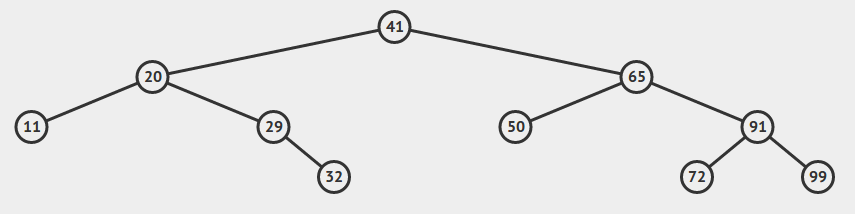
\includegraphics[width=0.8\textwidth]{img/BST}
  \end{center}
  \begin{itemize}
  \item \emph{Search Trees} Keep items in an ordered relationship.
  \item For example: Left children always have smaller values, Right
    children always have larger values;
  \item Insertion/Search/Deletion in a tree costs $O(h)$, where $h$ is
    the height of the tree;
  \item For a tree with $n$ elements, the \structure{minimum} height
    is $\text{log}n$
  \item For a balanced tree, the \structure{maximum} height is also
    $\text{log}n$
  \item How to keep the tree balanced?
  \end{itemize}
\end{frame}

\begin{frame}
  \frametitle{Balanced Search Trees}
  \framesubtitle{How to keep the tree balanced?}

  There are many Tree implementations/algorithms for keeping an BST
  balanced, and minimizing the tree height efficiently:
  \begin{itemize}
  \item AVL Tree (Adelson-Velskii-Landis);
  \item Red-Black Tree;
  \item B-Tree;
  \item Splay Tree;
  \end{itemize}
  \bigskip

  However, in a programming context (or even day to day life),
  implementing these trees from scratch is \alert{Dangerous}.

  \bigskip

  Luckly, most standard libraries include some implementation of BST.
\end{frame}

\begin{frame}
  \frametitle{ABLs in C++: Map and Set}

  \begin{itemize}
  \item In C++, the \emph{Map} and \emph{Set} classes are implemented
    using BSTs
  \item \emph{Map} Accept Key-value pairs;
  \item \emph{Set} Accepts only Keys;
  \end{itemize}

\end{frame}

\begin{frame}[fragile]
  \frametitle{Using Map in C++}
  {\small
\begin{verbatim}
#include <map>
map<string, int> ages;   ages.clear();

ages["john"] = 40;
ages["billy"] = 39;
ages["andy"] = 29;
ages["steven"] = 42;
ages["felix"] = 33;

// What is the age of andy?
map<string, int>::iterator it = ages.find("andy");
cout << it->second << endl;

// Which names are between "f" and "m" ??
for (map<string, int>::iterator it =
     age.lower_bound("f");              // finds felix
     it != age.upper_bound("m"); it++)  // finds johm
        cout << " " << ((string)it->first).c_str();
\end{verbatim}}
\end{frame}


\begin{frame}[fragile]
  \frametitle{Using Set in C++}
  {\small
\begin{verbatim}
#include <set>
set<int> CDs;
CDs.clear();

// Adding some values
CDs.insert(1000); CDs.insert(999); CDs.insert(1337);
CDs.insert(1313); CDs.insert(100020);

// Testing if a particular value exists (O(logn))
set<int>::iterator f = used_values.find(79);
if (f == used_values.end())
  cout << "not found!\n";
else
  cout << *f;    // Index!
\end{verbatim}}
\end{frame}

\subsection{Hash Tables}
\begin{frame}[fragile]
  \frametitle{Hash Tables}

  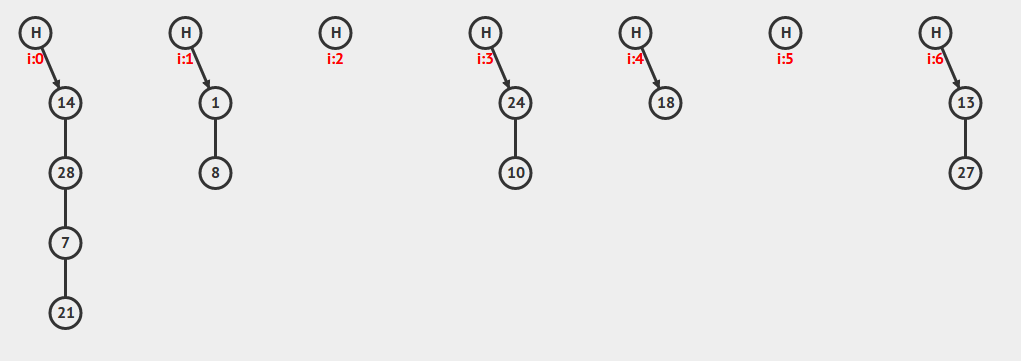
\includegraphics[width=0.95\textwidth]{img/hash}

  \begin{itemize}
  \item Insertion and Search: \structure{O(1)} -- \alert{Slow iteration};
  \item C++ library: \emph{std::unordered\_map};
  \item \structure{Hash} parameter -- Defines Collision results.
  \item Learn more about hash tables here: \url{https://visualgo.net/ja/hashtable}
  \end{itemize}
\end{frame}

\section{Other Data Structures}
\subsection{Motivation}
\begin{frame}
  \frametitle{Hand-making Data Structures}

  \begin{itemize}
  \item Sometimes, it is necessary to extend the standard data structures
    (arrays, maps, etc)
    \bigskip

  \item Other times, it is necessary to implement data structures not
    included in the standard libraries (graphs, UFDS, etc)
    \bigskip

  \item Let's see a few examples.
  \end{itemize}
\end{frame}

\subsection{Union-Find}
\begin{frame}
  \frametitle{Union-Find Disjoint Set (UFDS)}
  \framesubtitle{Motivating Problem}

  \begin{block}{Network Connections -- UVA793}
    In a network with $n$ computers, some are connected to others.\\
    \bigskip

    {\bf Input:} A series of ``commands''
    \begin{itemize}
    \item c i j -- Means computer $i$ is connected to computer $j$
    \item q i j -- Question: is computer $i$ connected to computer $j$?
    \end{itemize}

    \bigskip

    {\bf Output:} The number of ``q'' with answer yes, and the number
    of ``q'' with answer no.

  \end{block}
\end{frame}

\begin{frame}
  \frametitle{Union-Find Disjoint Set (UFDS)}
  \framesubtitle{Motivating Problem -- Naive answer}

  \begin{itemize}
  \item One idea: Use a Neighborhood Matrix $(n\times n)$ initalized with zeros.
  \item For every ``c i j'', $N_{i,j}, N_{j,i}$ becomes 1.
  \item We can follow the graph to answer ``q i j''.
  \end{itemize}

  \bigskip

  How good is this solution?
  \begin{itemize}
  \item Cost to insert a new connection: O(1)
  \item Cost to check if ``q i j'': O(n) (worst case)
  \end{itemize}

  \bigskip We can do better!
\end{frame}

\begin{frame}
  \frametitle{Union-Find Disjoint Set}

  \begin{center}
    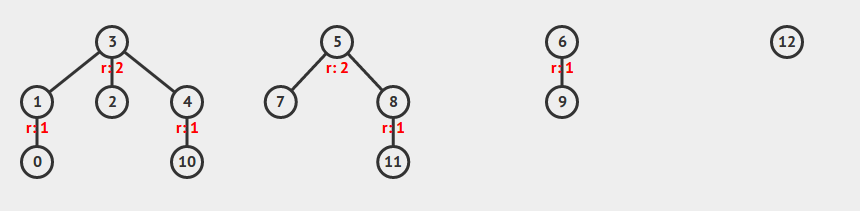
\includegraphics[width=.9\textwidth]{img/ufds1}
  \end{center}

  \begin{itemize}
  \item The UFDS keeps \structure{sets of items}, each is represented by a \structure{parent};
  \item When you join two sets \structure{You join their parents};
  \item When you test the parent of an item \structure{You flatten the tree};
  \item Test\_item and Join\_item are both O(1);
  \item More Information \url{https://visualgo.net/ja/ufds};
  \end{itemize}
\end{frame}

\begin{frame}[fragile]
  \frametitle{UFDS Implementation using Arrays}

  {\small
\begin{verbatim}
int p[MAX], r[MAX];
int find(int x) {
    return x == p[x] ? x : p[x]=find(p[x]);
}
int join(int x, int y) {
    x = find(x), y = find(y);
    if(x != y) {
        if(r[x] < r[y])
            p[x] = y, r[y] += r[x];
        else
            p[y] = x, r[x] += r[y];
        return 1;
    }
    return 0;
}
void init() {
    for(int i = 0; i < MAX; i++)
        p[i] = i, r[i] = 1; }

\end{verbatim}
}

\end{frame}

\begin{frame}
  \frametitle{Union Find Disjoint Set}
  \framesubtitle{Problem II -- War}
  {\small
  \begin{block}{}
    From a set of 10k people, some are friends, other are enemies.
    \begin{itemize}
      \item If A,B are friends, and B,C are friends, then A,C are friends
      \item If A,B are friends, and B,C are enemies, then A,C are enemies
      \item If A,B are enemies, and B,C are enemies, then A,C are friends
    \end{itemize}

    {\bf Input:} A series of commands from the set below:
    \begin{itemize}
    \item SetFriends(i,j)
    \item SetEnemies(i,j)
    \item TestFriends(i,j)
    \item TestEnemies(i,j)
    \end{itemize}

    {\bf Output:}
    \begin{itemize}
    \item If a ``SetFriends'' or ``SetEnemies'' is impossible, output ``-1''
    \item For a ``TestFriends'', ``TestEnemies'', output 0 - false, 1 - true
    \end{itemize}
  \end{block}}

\end{frame}

\begin{frame}
  \frametitle{Union Find Disjoint Set}
  \framesubtitle{Problem II -- War}

  This problem is similar to ``Networking'', but now you need to keep
  track of {\bf TWO} relations.

  \bigskip

  Some ideas:
  \begin{itemize}
  \item Keep UFDS for friends, and UFDS for enemies?
  \item Keep an ``enemy'' flag for each person?
  \item Add ``negative people'' to friend-set on UFDS?
  \end{itemize}

  \bigskip

  Which idea is easier to implement?
\end{frame}

\subsection{Segment Tree}
\begin{frame}[fragile]
  \frametitle{Range Maximum Query -- RMQ}

  Suppose you have an array of values:
\begin{verbatim}
Value: 18 17 13 19 15 11 20
Index:  0  1  2  3  4  5  6
\end{verbatim}

\bigskip

The \structure{Range Maximum Query} problem asks you to \structure{find
the index with the maximum value} between two indexes:

\begin{itemize}
  \item RMQ(0,0) = 0
  \item RMQ(0,6) = 6
  \item RMQ(1,4) = 3
\end{itemize}

\bigskip

\alert{Naive Method:} loop from $i$ to $j$, find maximum value. ($O(nk)$)\\
\medskip

But what is the number of {\bf Values} or {\bf Queries} is too big?
\end{frame}

\begin{frame}
  \frametitle{Segment Tree}

  \begin{itemize}
    \item Basic idea: \structure{index the array data in a binary tree}
    \bigskip

    \item Creation of the tree: \structure{$O(n)$}
    \bigskip

    \item Query of a segment: \structure{$O(\log n)$}
    \bigskip

    \item Update of the tree: \structure{$O(\log n)$} \hfill \alert{Important Part}
    \bigskip

    \item Many Implementations\\(this implementation: vector based heap)
  \end{itemize}
\end{frame}

\begin{frame}
  \frametitle{Segment Tree}
  \begin{center}
    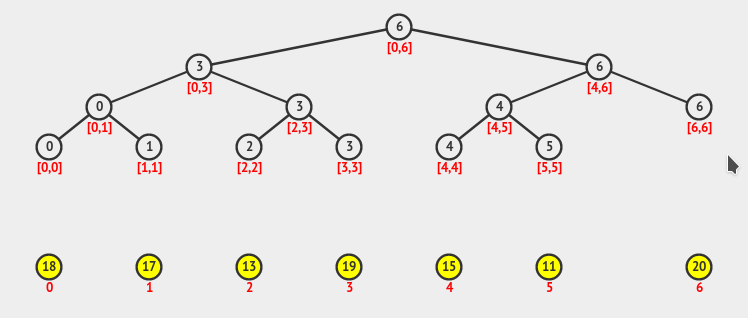
\includegraphics[width=1\textwidth]{img/segment_tree}
  \end{center}

  \bigskip

  Let's see the segment tree animation at VISUALGO.
\end{frame}

\begin{frame}[fragile]
  \frametitle{Coding the Segment Tree}
  \framesubtitle{Creating the Tree}
{\smaller
\begin{block}{}
\begin{verbatim}
typedef vector<int> vi; // We always use this!

class SegmentTree { // OOP implementation,
private: vi st, A;  // vi: typedef vector<int> vi;
  int n;
  int left (int p) { return  p<<1; }  // heap-like index;
  int right(int p) { return (p<<1) + 1; }

  void build(int p, int L, int R) {   // O(n log n)
    if (L == R)
      st[p] = L;                      // store the index
    else {                            // recursive build
      build(left(p) , L          , (L+R)/2);
      build(right(p), (L+R)/2 + 1, R      );
      int p1 = st[left(p)], p2 = st[right(p)];
      st[p] = (A[p1] <= A[p2]) ? p1 : p2;
  } }
\end{verbatim}
\end{block}}

\hfill\footnotesize{Code from \url{https://github.com/stevenhalim/cpbook-code}}

\end{frame}

\begin{frame}[fragile]
  \frametitle{Coding the Segment Tree}
  \framesubtitle{Query the Tree}
{\smaller
\begin{block}{rmq(1, 0, n-1, i, j) -- Query from i to j.}
\begin{verbatim}
int rmq(int p, int L, int R, int i, int j) // O(log n)
{
  if (i >  R || j <  L)
    return -1;    // outside query range
  if (L >= i && R <= j)
    return st[p]; // inside query range

  // compute the min position in the left and right part
  int p1 = rmq(left(p) , L        , (L+R)/2, i, j);
  int p2 = rmq(right(p), (L+R)/2+1, R      , i, j);

  if (p1 == -1) return p2;   // segment outside query
  if (p2 == -1) return p1;   // segment outside query
  return (A[p1] <= A[p2]) ? p1 : p2;
}
\end{verbatim}
\end{block}}
\hfill\footnotesize{Code from \url{https://github.com/stevenhalim/cpbook-code}}
\end{frame}

\begin{frame}[fragile]
  \frametitle{Coding the Segment Tree}
  \framesubtitle{Update the Tree}

{\smaller
\begin{block}{update(1, 0, n-1, i, v) -- update index i to value v}
\begin{verbatim}
int update(int p, int L, int R, int idx, int new_value) {
  int i = idx, j = idx;    //for point update i = j = idx
  // if the curr interval does not intersect the update,
  if (i > R || j < L) return st[p];  //return node value!
  // if the current interval is in the update range,
  if (L == i && R == j) {
    A[i] = new_value;     // update the underlying array
    return st[p] = L;     // this index
  }
  // compute the min pos in L/R part of the interval
  int p1, p2;
  p1=update(left(p) , L        , (L+R)/2, idx, new_value);
  p2=update(right(p), (L+R)/2+1, R      , idx, new_value);
  // return the position where the overall minimum is
  return st[p] = (A[p1] <= A[p2]) ? p1 : p2;
}
\end{verbatim}
\end{block}}
\hfill\footnotesize{Code from \url{https://github.com/stevenhalim/cpbook-code}}

\end{frame}



\section{}
\begin{frame}
  End of the Class!

  \vfill

  \begin{itemize}
    \item Questions about the problems?
    \bigskip

    \item Other questions?
  \end{itemize}
\end{frame}

\end{document}
